\chapter{Background Knowledge}
This chapter describes the theoretical background used in this thesis. It covers key aspects such as IoT, microcontrollers, wireless communication, cloud computing, Message Queue Telemetry Transport (MQTT), and their application in artwork tracking. Additionally, it addresses IoT security.

\section{Internet of Things}
IoT was first mentioned by the British technology pioneer Kevin Ashton in 1999 to describe a system, where sensors connect objects of the physical world to the internet \cite{Rose2015}. Today, the term is used to describe scenarios where internet connectivity and computing capabilities extend to a range of objects, devices, sensors, and everyday items \cite{Rose2015}. For instance, new IoT products such as internet-connected appliances, home automation components, and energy management devices are steering us towards a "smart home", offering enhanced security and energy efficiency \cite{Rose2015}. Other personal IoT devices, like wearable fitness and health monitoring devices, are revolutionizing the delivery of healthcare services \cite{Rose2015}. This technology is particularly promising for individuals with disabilities and the elderly, as it provides improved independence and quality of life at a reasonable cost \cite{Rose2015}. 

As shown in Figure 3.1 the number of IoT devices worldwide is projected to nearly double from 15.1 billion in 2023 to over 29 billion by 2030 \cite{Vailshery2023}. On one side, the increase in IoT devices is expected to offer economic and social benefits, including cost savings, value creation, productivity enhancements, and overall economic growth \cite{Castillo2015}. On the other, this growth could lead to a more sinister landscape filled with surveillance, privacy and security breaches, and consumer lock-in \cite{Rose2015}.

\begin{figure}[H]
  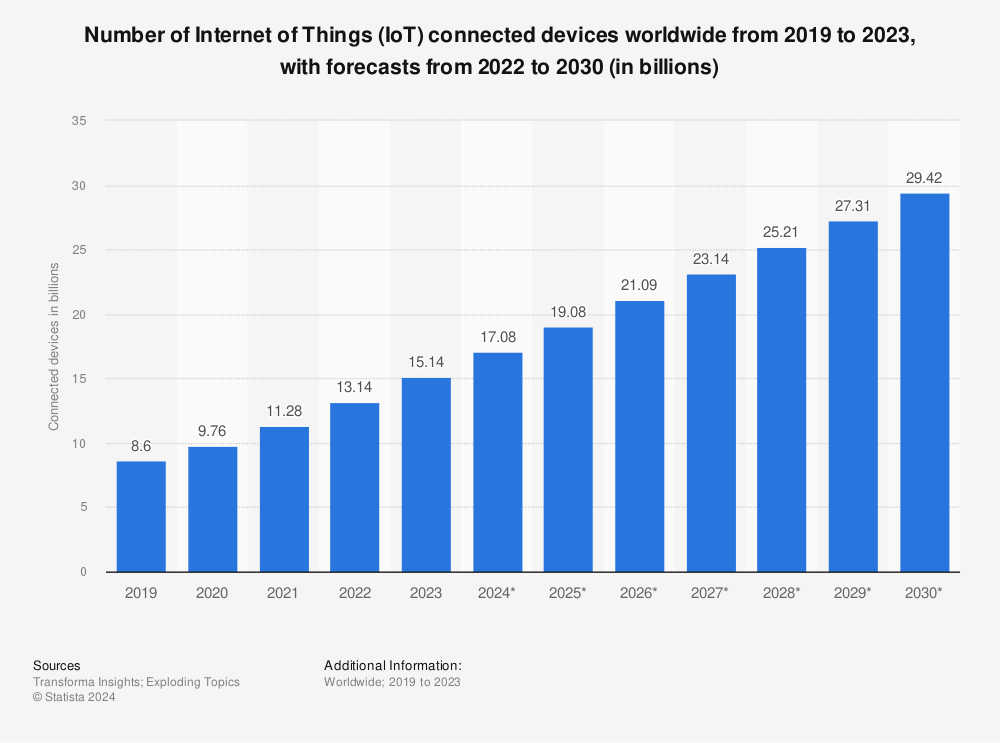
\includegraphics[width=\linewidth]{statistic_id1183457_number-of-iot-connected-devices-worldwide-2019-2023-with-forecasts-to-2030.png}
  \caption{Number of IoT connected devices worldwide from 2019 to 2023, with forecasts from 2022 to 2030, source: \cite{Statista2023}}
  \label{fig:Number of Internet of Things (IoT) connected devices worldwide from 2019 to 2023, with forecasts from 2022 to 2030}
\end{figure}

\section{Microcontroller}
What do mobile phones, control devices for automobiles, and monitoring and control systems for industrial automation have in common? - They are all embedded systems \cite{Lizarraga2006}.
Unlike general-purpose personal computers, embedded systems have specific requirements with pre-defined tasks to perform \cite{Lizarraga2006}.
The most popular type of an embedded system is a microcontroller, a compact computer system encapsulated within a single integrated circuit \cite{Lambert2017}.

STM32 microcontrollers are a range of microcontrollers that are divided into nine sub-families, and each one has its own set of features \cite{Noviello2017}. What they all do have in common is their Cortex-M core \cite{Noviello2017}. Cortex-M-based processors are a span of scalable, compatible, energy efficient, and easy-to-use processors designed for the low-cost-embedded market, suitable for IoT, connectivity, and smart metering applications \cite{Noviello2017}.
They also consist of a static RAM, flash memory, and debugging interface \cite{Noviello2017}.
There are some advantages for embedded developers to use the STM32 platform \cite{Noviello2017}.
Because of its Cortex-M-based processors and ARM's position in the embedded market, numerous tools are accessible to developers with ARM-based tool chains being completely free \cite{Noviello2017}.

The STMicroelectronics B-L462E-CELL1 Cellular Discovery Kit plays an important role in bringing IoT applications to life, especially those that require cellular connectivity and embedded sensor functionalities \cite{UM2743}.
The B-L462E-CELL1 board combines STM32 microcontroller technology with LTE cellular connectivity, allowing for the collection of sensor data and its transmission to remote cloud-based servers for further analysis and processing \cite{UM2743}.
Within the STM32 family, the B-L462E-CELL1 board utilizes the STM32L4 series microcontroller, which is known for its ultra-low-power capabilities \cite{UM2743}.
This microcontroller unit enables the connection of various sensors, such as the HTS221 which is shown in Figure 3.2. An ultra-compact sensor for measuring relative humidity from 20 to +80\% rH, with an accuracy of +- 3.5\% rH, and temperature from +15 to +$40^\circ$C, with an accuracy of +- $0.5^\circ$C \cite{DS10329, UM2743}.
Another sensor is the LSM303AGR, which is an ultralow-power high-performance system-in-package with a 3-axis digital linear acceleration sensor, which measures the acceleration on the x-, y- and z-axis and returns the data in mg \cite{DS10999}.
Furthermore, the integration of LTE cellular connectivity, by utilizing its built-in eSIM or an extern SIM by using the SIM card slot shown in Figure 3.2, provides a method for transmitting sensor data to cloud-based servers. This feature is essential for applications that require real-time or periodic transmission of sensor data to remote servers for monitoring, and analysis\cite{UM2743}.

\begin{figure}[h]
  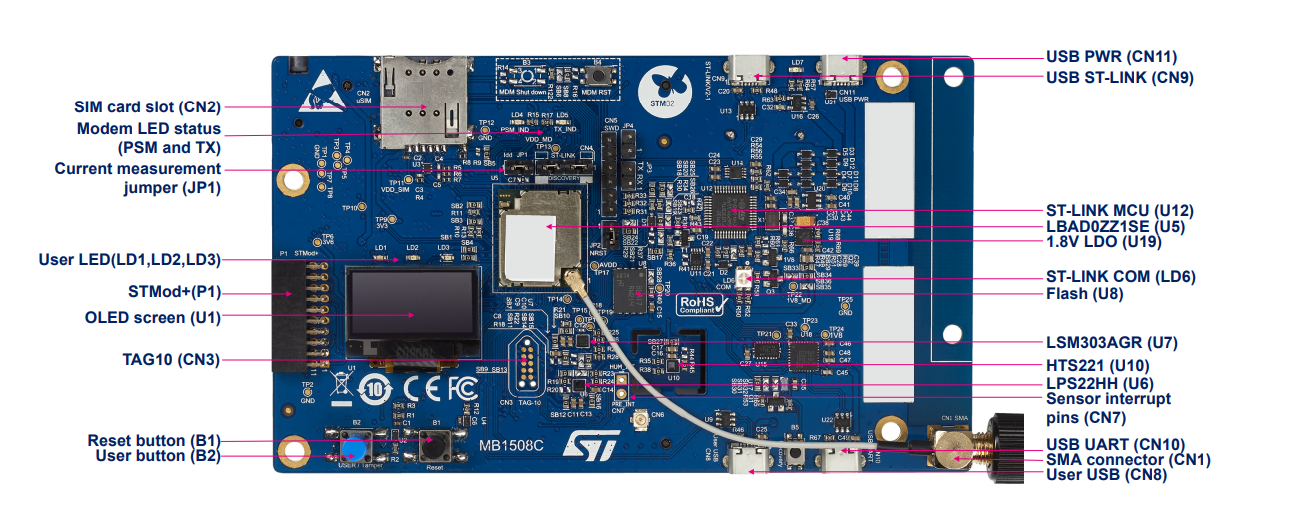
\includegraphics[width=\linewidth]{B-L462E-CELL1_Front.png}
  \caption{B-L462E-CELL1 Discovery kit (top view), source: \cite{UM2743}}
  \label{fig:B-L462E-CELL1 Discovery kit (top view)}
\end{figure}

Figure 3.3 illustrates that the B-L462E-CELL1 board can also be battery-operated, making it useful for systems on the move where access to power sources may be limited or unavailable.

\begin{figure}[H]
  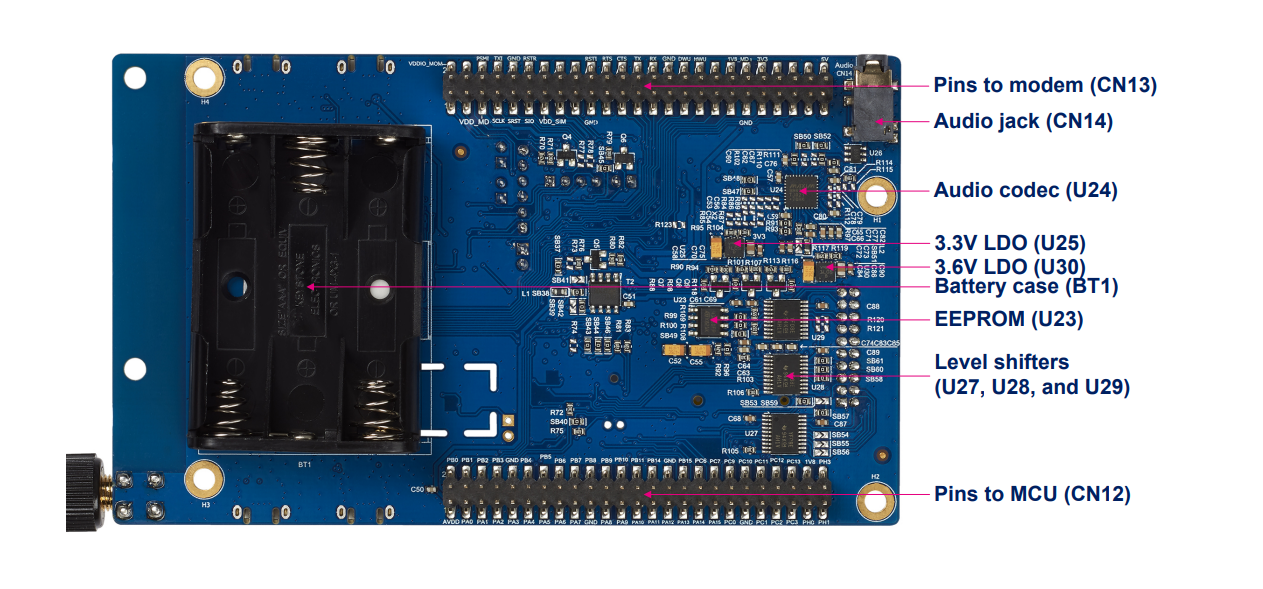
\includegraphics[width=\linewidth]{B-L462E-CELL1_Back.png}
  \caption{B-L462E-CELL1 Discovery kit (bottom view), source: \cite{UM2743}}
  \label{fig:B-L462E-CELL1 Discovery kit (bottom view)}
\end{figure}

\section{Wireless Communication Technologies}
LTE is a standard for wireless broadband communication for mobile devices and data terminals, developed by the 3rd Generation Partnership Project (3GPP) \cite{TutorialspointLTE, ThalesgroupLTE}. It is the evolution of the Universal Mobile Telecommunication System (UMTS), which evolved from the Global System for Mobile Communications (GSM) \cite{TutorialspointLTE}.

LTE provides high data rates, low latency, and a packet-optimized radio access technology that supports flexible bandwidth deployments \cite{TutorialspointLTE}. It is an ideal technology for supporting high data rates for services such as Voice over IP (VoIP), streaming multimedia, video conferencing, or as a high-speed modem for mobile devices \cite{TutorialspointLTE}. LTE uses both Time Division Duplex (TDD) and Frequency Division Duplex (FDD) modes \cite{TutorialspointLTE}.

In the context of IoT, LTE provides a reliable connection for IoT devices to complete data transfers to the cloud and other devices \cite{TelitLTE}. It also enables cellular LPWA (Low Power Wide Area) networks (e.g., Cat M and NB-IoT) to operate on its infrastructure \cite{TelitLTE}.

LTE-M, also known as LTE Cat-M1, is a type of Low-Power Wide-Area Network (LPWAN) radio communication technology developed by 3GPP for machine-to-machine and IoT applications \cite{TelekomLTE}. LTE-M was designed for cost-effective IoT applications, using low data rates, requiring long battery life, and often operated in locations that are hard to reach \cite{TelenorLTE}.

\section{Cloud Computing}
Cloud computing is when computing resources are delivered over the internet \cite{Investopedia2023}. It allows access to computing resources, such as storage and infrastructure, which removes the need for individuals to manage physical resources, such as servers, independently, allowing them to pay only for what they use \cite{GoogleCloud}. There are three types of cloud computing, public -, private -, and hybrid clouds \cite{GoogleCloud}. Public Clouds are made available by third parties, offering computing, storage, and network resources over the internet \cite{GoogleCloud}. Private clouds are privately hosted in their data centers, which makes them more secure \cite{GoogleCloud}. Hybrid clouds combine the other two types, using the advantages of both \cite{GoogleCloud}.

One example of a public cloud is AWS IoT Core, which lets connected devices interact with cloud applications and other devices \cite{EMQTechnologies}. It offers multiple communication protocols, including MQTT and HTTPS \cite{AWS}. It also provides secure communication between devices by using authentication and end-to-end encryption \cite{AWS}.

\section{Message Queue Telemetry Transport}
A protocol is a special set of rules and regulations in a telecommunication connection, that endpoints use to communicate to other endpoints connected to the same network \cite{Kraijak2015}. 
One of these protocols is MQTT, a standardized publish/subscribe protocol, released by IBM in 1999 \cite{Soni2017}. It was planned to send data accurately under long network delays and low-bandwidth network conditions \cite{Soni2017}.

As Figure 3.4 illustrates, several devices (subscribers) subscribe to a topic, for example, "temp", on an MQTT broker \cite{OPC}. A publisher, such as an IoT device, can then publish its data, such as the measured temperature, to the broker \cite{OPC}. The broker then traverses his subscription list and sends the data to the subscribers of "temp" \cite{OPC}.

\begin{figure}[H]
  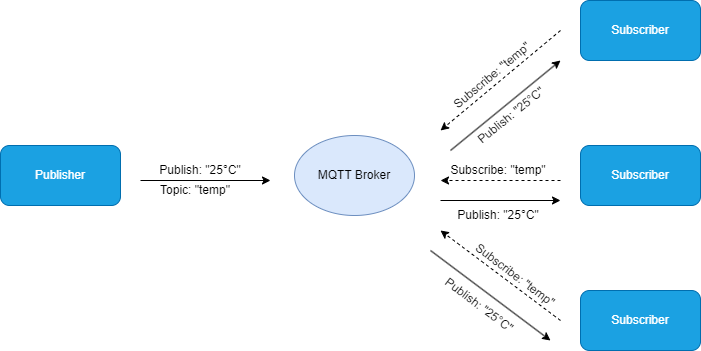
\includegraphics[width=\linewidth]{MQTT_Diagram.png}
  \caption{Diagram illustrating the operation of the MQTT protocol}
  \label{fig:Diagram illustrating the operation of the MQTT protocol}
\end{figure}

MQTT also has its limitations, one of them being message expiration, where messages that are not gathered from the broker will stay there forever, resulting in an overload of the broker, which degrades the overall performance \cite{Soni2017}. While message delivery is guaranteed, there is no guarantee that the order of the messages is correct, making it important to add timestamps to the messages \cite{Soni2017}.

\section{Artwork Tracking}
Artwork monitoring is one of many IoT applications. It involves IoT devices to track and monitor environmental parameters such as temperature and humidity, which are crucial for the preservation of artwork. Several studies have proposed IoT monitoring systems. 

For instance, \cite{Fort2022} discusses their work on health monitoring for artwork and large wood structures. They employed an STM32 to measure temperature, humidity, and tilt. They explored two scenarios: one static and one mobile. In the static scenario, measurement nodes transmit data via BLE to BLE Gateways, which connect to a Modem or a Switch \cite{Fort2022}. From there, the data is sent either over the internet or the local network to a remote cloud and database or a local server \cite{Fort2022}. In the mobile scenario, measurement nodes send data via Bluetooth Low Energy (BLE) to a smartphone or tablet acting as a gateway, which then transmits the data via cellular network to the Cloud \cite{Fort2022}.

Furthermore, \cite{Hinostroza2022} focuses on environmental monitoring of cultural heritage, measuring temperature, humidity, and light intensity. Their setup involves measurement nodes sending data to a central Node via BLE or ZigBee, with the central node transmitting the data via WiFi or General Packet Radio Service (GPRS) to the Cloud.

\section{Security}
Security is a big concern in the field of IoT. As IoT devices proliferate as shown in Figure 3.1, so do the potential vulnerabilities and security risks. \cite{Noor2019} delves into the security aspects of IoT devices, providing a comprehensive overview of the challenges and solutions associated with each layer of the IoT architecture:

The IoT architecture is typically based on a 3-layer system: the Perception/Hardware Layer, the Network/Communication Layer, and the Application (Interface/Service) Layer. Each of these layers has its own set of vulnerabilities and corresponding solutions.

The perception/hardware layer is the first line of defense in an IoT system. This layer is often filled with hardcoded credentials, a significant issue that poses a risk due to the widespread use of the same password across multiple devices. This makes devices prone to unauthorized access and manipulation.

The network/communication layer is responsible for transmitting the data collected by the hardware to the application layer. Authentication emerges as a key strategy for securing communication within this layer. By ensuring that only authorized devices can connect and transmit data, the integrity and confidentiality of the data can be maintained.

The application layer is where the data is processed and presented to the end-user. This layer benefits from biometrics and multi-level authentication to keep bad actors from modifying configurations. By implementing robust authentication mechanisms, unauthorized access to the system can be prevented, thereby protecting the data and the system as a whole.

In conclusion, securing IoT devices is a complex task that requires a multi-layered approach. By understanding the vulnerabilities of each layer and implementing the appropriate security measures, the integrity and security of IoT systems can be significantly enhanced.

One security measurement, for the network/communication layer, would be a Virtual Private Network (VPN). It provides secure connections between the endpoints of the devices, by establishing secure tunnels to send and receive encrypted data \cite{JUMA2020102598}. One of the most common VPN security protocols for IoT devices is the Internet Protocol Security (IPSec/IPv6), which encrypts data through static IP addresses ensuring privacy and End-to-End secure communication through public Internet traffic \cite{JUMA2020102598}.